\section{Vårt Arbeid}

\subsection{Utstyrsliste} % Må da finnes en penere måte

Veroboard, 32 sockets

Kretskort gitt til lab i TFE4101

Digital Oscilloskop - Rohde \& Schwarz RTB2004

Signalgenerator - Rohde \& Schwarz HMF2525

Spenningskilde - Rohde \& Schwarz HMC 8042

Banankabler

BNC-BNC kabler

BNC-banankabel

BNC-splitter

Prober

\subsection{Forarbeid}

\subsubsection*{Design av absoluttverdikrets}

I forarbeidet skulle det designes en 4-bits absoluttverdikrets.
For å ta absoluttverdien av et binært tall kan man invertere det og addere 1.
En absoluttverdikrets kan dermed bygges opp av inverterkretser og av halvadderkretser.
Vi startet med å designe en inverterkrets, altså en krets som inverterer hvert bit som kommer inn, hvis kretsen er aktivert.

Det blir gjort tydelig av tabell \ref{tabell:1} at en slik krets kan lett implementeres som en XOR-port.

\begin{table}[h]
  \centering
  \begin{tabular}{c c|c}

    In & En & Out\\
    \hline
    0 & 0 & 1\\
    0 & 1 & 0\\
    1 & 0 & 1\\
    1 & 1 & 0\\

  \end{tabular}
  \caption{Sannhetstabell for inverterkrets}
  \label{tabell:1}
\end{table}

% \begin{figure}
%   \centering
%   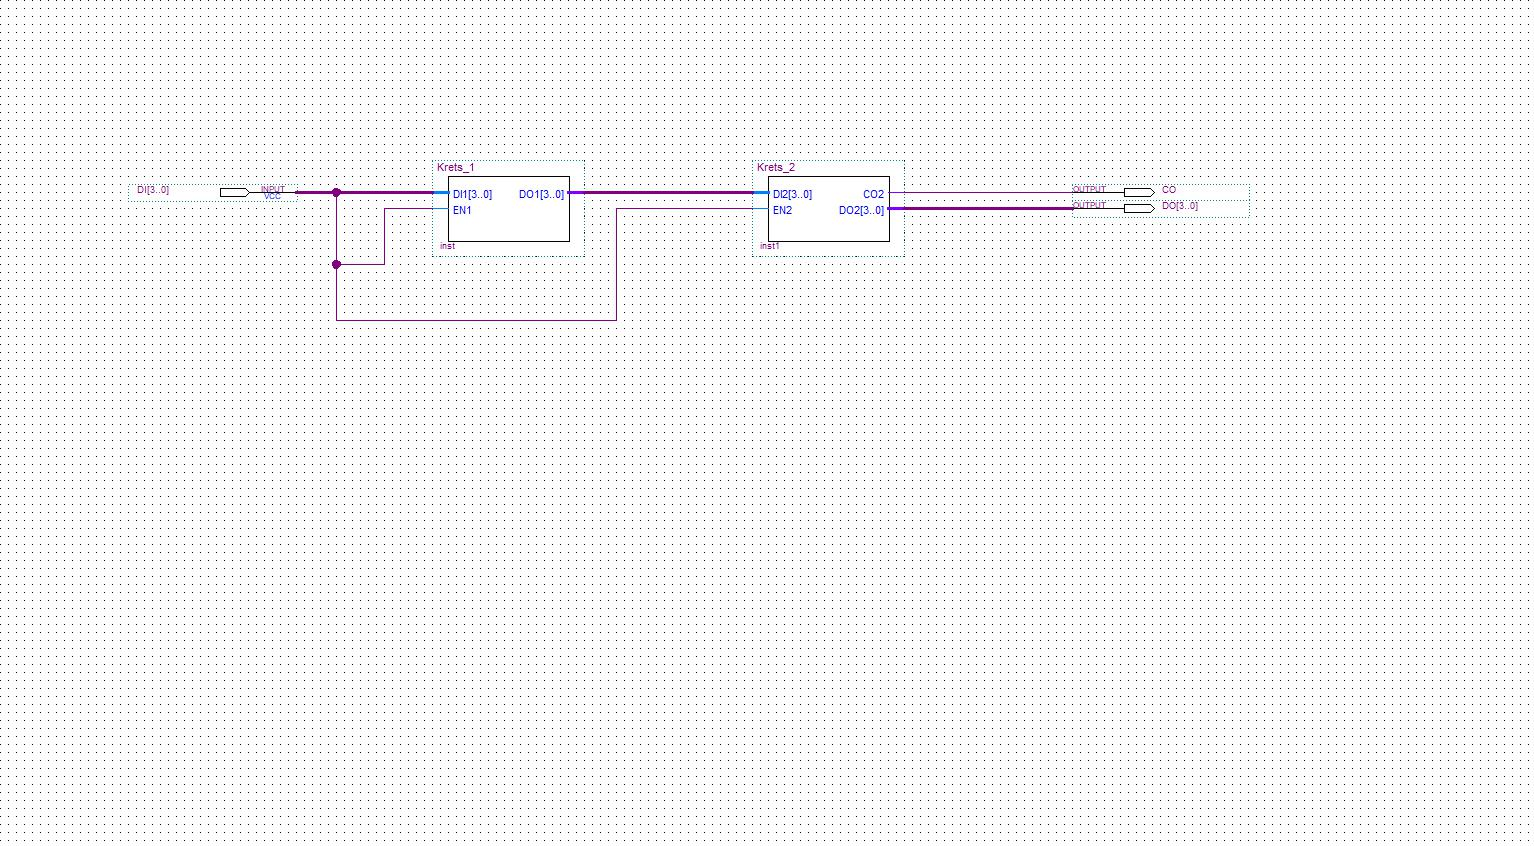
\includegraphics{4 bit abs}
%   \caption{}
%   \label{}
% \end{figure}

Deretter designet vi en halvadderkrets. En halvadderkrets adderer to tall og har to utganger, en for summen og en for mente, så lenge kretsen er aktivert.

\begin{table}[h]
  \centering
  \begin{tabular}{c c|c|c}

    In & Carry-In & Sum & Carry-Out\\
    \hline
    0 & 0 & 0 & 0\\
    0 & 1 & 1 & 0\\
    1 & 0 & 1 & 0\\
    1 & 1 & 0 & 1\\

  \end{tabular}
  \caption{Sannhetstabell for halvadderkrets}
  \label{tabell:2}
\end{table}

% \begin{figure}
%   \centering
%   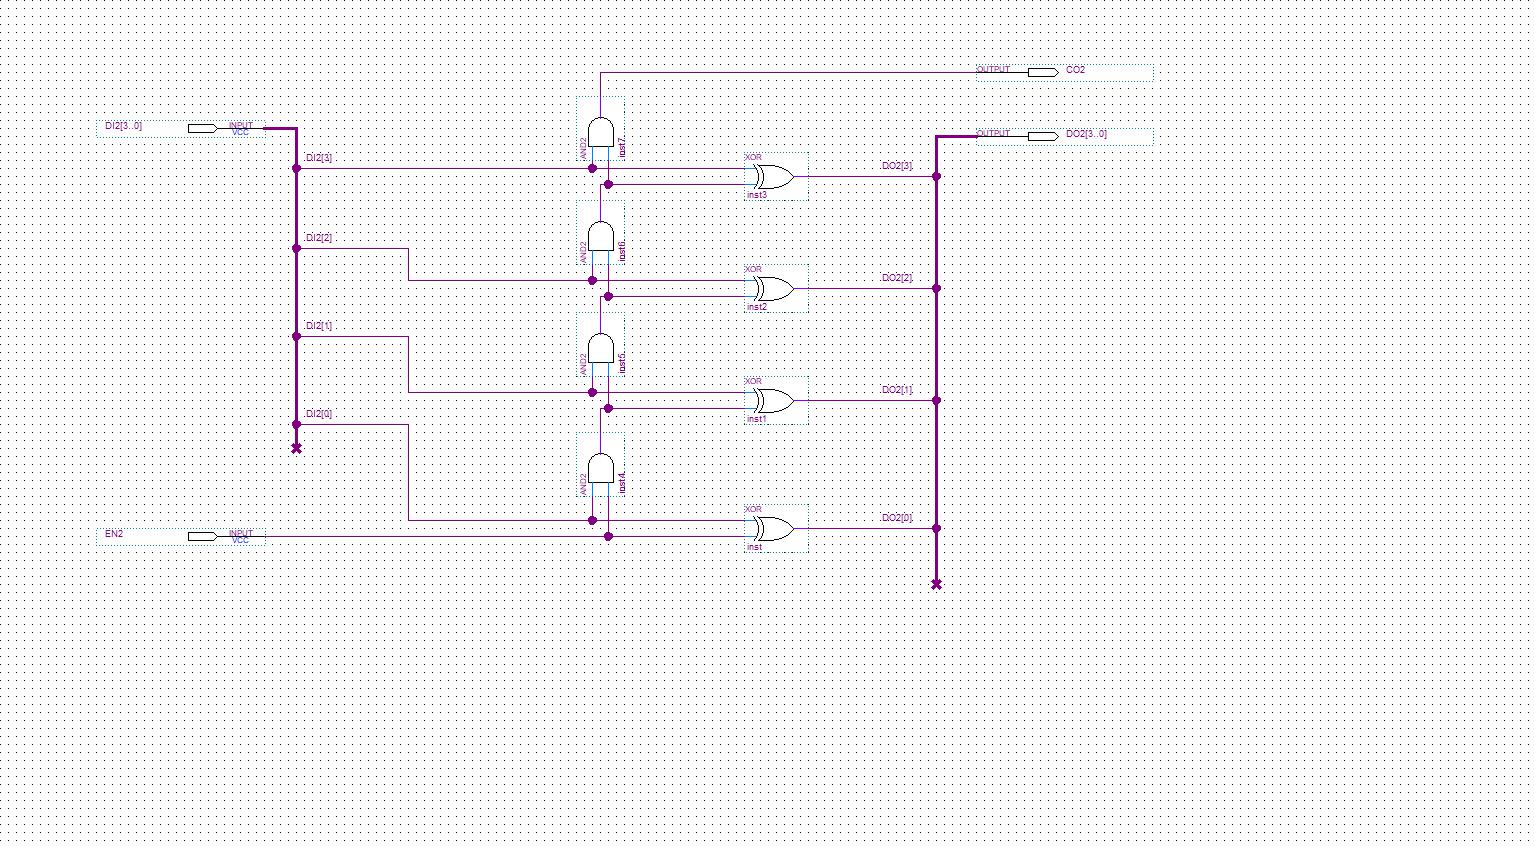
\includegraphics{4 bit adder}
%   \caption{}
%   \label{}
% \end{figure}

Etter å ha designet disse komponentene, måtte vi sette de sammen til å bli en 4-bits absoluttverdikrets.
Da lagde vi blokker ved å sette inverterkretsen og halvadderkretsen i serie, og satte fire av disse blokkene i parallell.
Videre brukte vi MSB som enable signal for inverterne og som mente inn for første halvadder, slik som i figur [REF HER].

\subsubsection*{Beregning av kritisk sti og maksimal klokkehastighet}

Kritisk sti fant vi ved å se på det scenarioet hvor det blir flest menteforplantninger, nemlig overgangen fra 1000 til 1000, hvor det skjer menteforplantninger gjennom hele kretsen.
Da går kritisk sti gjennom 2 XOR porter og 3 AND porter.
For å beregne forsinkelsen gjennom kritisk sti fant vi verdiene for forsinkelse gjennom de forkjellige portene ved 5V som maks spenning, som er som gitt i Tabell \ref{tabell:3}

\begin{table}[h]
  \centering
  \begin{tabular}{c c}

    Port & Forsinkelse\\
    \hline
    AND & 125ns\\
    XOR & 140ns\\

  \end{tabular}
  \caption{Forsinkelsestid gjennom porter}
  \label{tabell:3}
\end{table}

Gitt disse verdiene kan vi regne oss frem til forsinkelse gjennom kritisk sti.

\begin{displaymath}
  2 \cdot 140ns + 3 \cdot 125ns = 655ns
\end{displaymath}

Dette gir oss at maksimal klokkehastighet er... SJEKK VERDI

\begin{displaymath} % SJEKK VERDI
  1/655ns = \SI{1.53}{\mega\hertz}
\end{displaymath}

\clearpage

\subsection{Kobling av absoluttverdikrets}
